\chapter{差分隐私}\label{chap:differential-privacy}
\begingroup
\newcommand{\pref}{Chapters/differential-privacy/figures}

在本章我们关心数据的另一个维度:社会属性. 机器学习需要大量的数据,这些数据从何而来?大部分时候,是通过收集个体的数据得到的. 于是这里就涉及到了隐私的问题,如何保护个体的隐私,同时又能够让机器学习得到足够的数据?\textbf{差分隐私}\index{差分隐私}就是解决这个问题的一个方法,本章将更详细地介绍差分隐私的概念和应用. 

\section{数据隐私问题}

许多科研工作的开展和推进都需要有大量真实有效的数据作为支撑. 以医学为例,我们需要大量真实的病人提供病情数据. 但这些数据可能都涉及到病人的隐私信息,例如一些\emph{敏感数据}. 因此,我们必须找到一种方法,既可以收集到这些数据,又保护病人的隐私信息.

保护病人的隐私信息的一种理解是不会让数据获得者将数据和人对应起来. 那么最直观的想法就是将每条\emph{数据匿名化}\index{数据匿名化}. 比如,每条数据只包含患者的生日、性别、邮政编号(代表位置)、病情. 这样做依然有问题:同一天生日、同一性别、相同邮政编号的人很少,而这些信息很容易被找到,比如公开的选民名册. 于是通过一条数据的各种属性可以轻易定位到这个人,这样的匿名化是不安全的.

我们再看一个例子。2006年,Netflix 举办了关于电影推荐系统的算法设计比赛.
只公开了匿名代号和对应用户的观看电影名称、打分的数据集(这次连生日、性别都没有). 但这一数据集很快被破解,问题出在只要对某个用户稍微熟悉一些,就很容易对应出这个用户和观影数据. 这种破解让部分用户感到焦虑,例如性少数群体害怕其他人可以从自己的观影记录中判断出自己的性取向. 第二届Netflix Prize 竞赛也因此停办.

这两个例子展现的是一种\emph{去匿名化}\index{去匿名化}的现象,也就是说匿名的数据实际上揭示了数据对应的那个个体。这去匿名化的出现都是因为数据具有\emph{独特性}. 比如我们看\Cref{tab:tab01},这是医院甲的病人数据表。56岁的病人只有Rebecca,所以假如我们知道Rebecca的年龄并了解到她去过这家医院,便立即得知她患有HIV.

\begin{table}[!ht]
\centering
\begin{tabular}{cccccc}
    \toprule
    \textbf{姓名} & \textbf{年龄} & \textbf{性别} & \textbf{邮政编码} & \textbf{是否吸烟} & \textbf{诊断} \\ \midrule
    李国强 & 64 & 男性 & 190146 & 是 & 心脏病 \\ 
    王秀英 & 61 & 女性 & 190118 & 否 & 关节炎 \\ 
    张建华 & 67 & 男性 & 190104 & 是 & 肺癌 \\ 
    陈玉兰 & 63 & 女性 & 190146 & 否 & 克罗恩病 \\ 
    刘志强 & 69 & 男性 & 190115 & 是 & 肺癌 \\ 
    赵丽娜 & \light{56} & 女性 & 190103 & 否 & 艾滋病 \\ 
    周志成 & 52 & 男性 & 190146 & 是 & 糖尿病 \\ 
    马文杰 & 59 & 男性 & 190130 & 是 & 过敏性鼻炎 \\ 
    李梅 & 55 & 女性 & 190146 & 否 & 溃疡性胃炎 \\ \bottomrule
    \end{tabular}

\caption{医院甲的病人数据表。}
\label{tab:tab01}
\end{table}

一种减少\emph{独特性}的思想是\emph{$k$-匿名性}\index{$k$-匿名性}:任何一个人的信息都不能和其他至少$(k-1)$人区分开. 比如,可以不明确写出姓名、年龄和邮编,只给出模糊的范围,于是数据变成了下面的\Cref{tab:tab02}.

\begin{table}[!ht]
\centering
\begin{tabular}{cccccc}
\toprule
    \textbf{姓名} & \textbf{年龄} & \textbf{性别} & \textbf{邮政编码} & \textbf{是否吸烟} & \textbf{诊断} \\ \midrule
    * & 60-70 & 男 & 1901** & 是 & 心脏病 \\ 
    * & 60-70 & 女 & 1901** & 否 & 关节炎 \\ 
    * & 60-70 & 男 & 1901** & 是 & 肺癌 \\ 
    * & 60-70 & 女 & 1901** & 否 & 克罗恩病 \\ 
    * & 60-70 & 男 & 1901** & 是 & 肺癌 \\ 
    \light* & \light{50-60} & \light{女} & \light{1901**} & \light{否} & 艾滋病 \\ 
    * & 50-60 & 男 & 1901** & 是 & 糖尿病 \\ 
    * & 50-60 & 男 & 1901** & 是 & 过敏性鼻炎 \\ 
    \light* & \light{50-60} & \light{女} & \light{1901**} & \light{否} & 溃疡性胃炎 \\ \bottomrule
\end{tabular}

\caption{医院甲的病人数据表,模糊了姓名、年龄和邮编。}
\label{tab:tab02}
\end{table}

这种方法仍然存在问题,因为我们不能把关键信息(病症信息)也模糊化. 如果我们还拿到了另一家医院乙的模糊之后的病人数据表(\Cref{tab:tab03}),那么依然有办法定位到Rebecca:这两张表上50-60岁的女性只有HIV是重合的,如果我们知道Rebecca的年龄并知道她同时去过两家医院,便立即得知她患有HIV.

\begin{table}[!ht]
\centering
\begin{tabular}{ccccc}
    \toprule
    \textbf{姓名} & \textbf{年龄} & \textbf{性别} & \textbf{邮政编码} & \textbf{诊断} \\\midrule
    * & \textcolor{Orchid}{50-60} & \textcolor{Orchid}{女} & 1901** & 艾滋病 \\ 
    * & \textcolor{Orchid}{50-60} & \textcolor{Orchid}{女} & 1901** & 系统性红斑狼疮 \\ 
    * & \textcolor{Orchid}{50-60} & \textcolor{Orchid}{女} & 1901** & 干燥综合征 \\ 
    * & 60-70 & 男 & 1901** & 胰腺癌 \\ 
    * & 60-70 & 男 & 1901** & 肝硬化 \\ 
    * & 60-70 & 男 & 1901** & 通风 \\ \bottomrule
    \end{tabular}
\caption{医院乙的病人数据表,模糊了姓名、年龄和邮编。}
\label{tab:tab03}
\end{table}

除了使用匿名化的手段,还有一种方法可以保护隐私:不再提供单人的数据,而是直接公布将数据集的总体信息,比如平均值. 但这种方法也不一定能保证不泄露单人数据. 例如:我们只公布一个机器学习模型(这算是一直非常抽象的总体信息). 很多研究表明可以通过尝试不同的测试数据来判断出这个机器学习模型的训练集,这是因为机器学习模型总是会偏向于过拟合训练集数据. 所以如果对某个测试数据的结果很有自信,往往说明这一数据存在于训练集中. \lhysays{给一个ref}

\begin{remark}
以上这些内容都说明\textbf{匿名化}很难保护个人隐私. 那么是否可以使用密码学的手段进行\textbf{加密}?其实加密和隐私在出发点上完全不同. 加密的目的是为了不让别人获取到真实数据. 而隐私是一个比简单地锁定数据更微妙的问题——我们希望我们的算法的结果能够释放有用的信息,而不是泄露私人信息. 因此我们这里讨论的其实是隐私保护问题而不是加密问题。
\end{remark}

\section{差分隐私的定义与性质}

我们上面探讨了隐私保护的必要性以及它的微妙之处,现在我们要给出一种合理的方案解决隐私保护的问题,这个方案就是\emph{差分隐私}。要给出一个数学模型,不仅要知道什么情况下算是隐私泄漏,也需要知道什么情况下不算,所以我们再来看一个反面的例子。

Broky是一位长期吸烟的男子,他参加了一项有关“吸烟与健康”的调查. 这项调查在不久后发布了一项结果,表明长期吸烟的人患上肺癌的几率更大. 伴随着这一结果的公布,保险公司在出售相同保险时会对长期吸烟者索要更高的价格. Broky当然也受到了这一政策的影响. 那我们是否可以认为这项研究泄露了Broky(更有可能患病)的隐私呢?

我们的直观应该是不算泄露了隐私. 因为“长期吸烟的人患上肺癌的几率更大”这项结论并不依赖于Broky是否参加了调查. 考虑这样的对照,$x$代表原来参加调查的人的集合,$x'$代表其他人不变,只是Broky换成了另外一个人的集合. 如果是$x'$这些人参与了调查,结论是否会发生变化?\emph{大概率}不会!

Broky的例子告诉我们对于隐私的一种合理的衡量应该有以下性质:\emph{当数据集中包含Broky的信息,相比数据集中不包含Broky的信息,并不会\textbf{明显}增加损害Broky的利益的概率.} 这一思想引出了\emph{差分隐私}\index{差分隐私}的概念,我们将在下面给出数学形式的定义.

考虑数据的空间$\mathcal X$,其中的每一个元素都包含了个体的所有可能数据例如姓名、性别、年龄、国籍等. 考虑$n$个人的数据,形成了有序的数据集$x = (x_1, \cdots, x_n) \in \mathcal X^n$.  设 $A$ 是一种随机算法:在固定输入数据集 $x \in \mathcal X^n$下,$A(x)$ 是结果空间 $\mathcal Y$ 上的一个随机变量. 当我们改变(增加或删除)一个人的数据时,我们希望结果分布的变化可以控制在一定范围内. 为此,我们引入相邻数据集的概念:

\begin{definition}[$k$-相邻数据集]\index{$k$-相邻数据集}
    设 $x, x' \in \mathcal X^n$,如果 $x$ 和 $x'$ 最多有$k$条数据不同,即至多存在$k$个不同的$i_1,\dots,i_k \in [n]$ 使得 $x_{i_j}=x_{i_j}'$对$j\in[k]$成立,那么称 $x$ 和 $x'$ 是 $k$-相邻的.
\end{definition}

在之前的例子中,含有Broky的被调查者的数据集和把Broky换为任意一个其他人的数据集时$1$-相邻数据集.

现在我们给出差分隐私的定义。

\begin{definition}[$\epsilon$-DP]\index{$\epsilon$-DP}
考虑随机算法 $A : \mathcal X^n \to \mathcal Y$,如果对于任一对$1$-相邻数据集$x, x'$,对任意(可测)值集 $E \subseteq \mathcal Y$,有
\[
\Pr(A(x)\in E) \leq e^{\epsilon} \cdot \Pr(A(x')\in E),
\]
那么我们称$A$为\emph{数据集大小为 $n$ 的 $\epsilon$-DP算法}.
\end{definition}

需要注意的是,这一定义是针对随机算法的,并且是对称的,也就是$x$和$x'$的地位是平等的。直观上一个,$\epsilon$-DP算法的输出分布在相邻数据集上的变化不会太大. $\epsilon$衡量的是信息的泄漏量;$\epsilon$越大,算法泄漏的信息就越多,隐私保护效果当然也变差.

以上定义需要对所有的(可测)值集$E$都成立,这给验证带来了极大的困难,如果随机算法的输出分布是更加常规的,我们可以简化验证的过程. 

对于离散型的输出,我们有如下等价定义:
\begin{proposition}\label{prop:discrete-dp}
    如果 $A(x)$对于任意 $x \in \mathcal X^n$ 都是离散型随机变量,那么随机算法$A$是数据集大小为 $n$ 的 $\epsilon$-DP算法,当且仅当对于任意一对$1$-相邻数据集$x, x'$和所有的 $y \in \mathcal Y$,有
    \[
    \Pr(A(x) = y) \leq e^{\epsilon} \cdot \Pr(A(x') = y).
    \]
\end{proposition}
\begin{proof}
$\implies$:取$E = \{y\}$即可证明.

$\impliedby$:假设$E=\{y_1,\dots,y_k,\dots\}$. 对每一个$y_i$,都有
    \[
    \Pr(A(x) = y_i) \leq e^{\epsilon} \cdot \Pr(A(x') = y_i).
    \]
因为$A(\cdot)=y_i$对于不同的$i$是互斥事件,所以概率可以直接相加,于是:
    \[
    \Pr(A(x) \in E) = \sum_i \Pr(A(x) = y_i) \leq e^{\epsilon} \cdot \sum_i\Pr(A(x') = y_i) = e^{\epsilon} \cdot \Pr(A(x') \in E).
    \]
\end{proof}

对连续型的输出,我们有如下等价定义:
\begin{proposition}\label{prop:continuous-dp}
如果 $A(x)$对于任意 $x \in \mathcal X^n$ 都是连续型随机变量,那么它存在概率密度函数,记为$h_{x}$. 此时随机算法$A$是数据集大小为 $n$ 的 $\epsilon$-DP算法,当且仅当对于任意一对$1$-相邻数据集$x, x'$和几乎所有的 $y \in \mathcal Y$,有
    \[
    h_{x}(y) \leq e^{\epsilon} \cdot h_{x'}(y).
    \]
\end{proposition}
\begin{proof}\footnote{这一部分的严格表述需要测度论的基础,所以这一证明从直观上理解即可,不需要考虑严格的定义。}
$\implies$:根据概率密度函数的定义(实际上是Lebesgue微分定理),对$x\in\mathcal X^n$,取$E_\delta = (y-\delta, y+\delta)$,对几乎所有的$y\in\mathcal Y$,有
\[\frac{\d}{\d\delta}\Pr(A(x)\in E_\delta)=h_x(y).\]
因此,对几乎所有的$y\in\mathcal Y$,
\[\forall\delta>0\,\Pr(A(x)\in E_\delta) \leq e^{\epsilon} \cdot \Pr(A(x')\in E_\delta)\implies h_x(y)\leq e^\epsilon\cdot h_{x'}(y).\]
$\impliedby$:依然根据概率密度函数的定义,考虑$x,x'\in\mathcal X^n$,对任意可测$E\subseteq\mathcal Y$,有
\[\Pr(A(x)\in E)=\int_E h_x(y)\d y\leq e^\epsilon\cdot\int_E h_{x'}(y)\d y=e^\epsilon\cdot\Pr(A(x')\in E).\]
\end{proof}

接下来我们给出差分隐私的基本性质。

\begin{proposition}[复合性,两个算法的情形]\label{prop:composition}\index{差分隐私!复合性}
    $A_1$ 和 $A_2$ 是相互独立的随机算法,其中 $A_1 : X^n \to \mathcal Y_1$,$A_2 : \mathcal Y_1 \times \mathcal X^n \to \mathcal Y_2$. 假设$A_1$是 $\epsilon_1$-DP算法,$A_2$ 是 $\epsilon_2$-DP算法.
    
    令 $A :\mathcal X^n \to \mathcal Y_1 \times \mathcal Y_2$ 是随机算法,输出为 $A(x) = (y_1, y_2)$,其中 $y_1 = A_1(x)$, $y_2 = A_2(y_1, x)$,那么 A 是$(\epsilon_1 + \epsilon_2)$-DP算法.
\end{proposition}

\begin{proof}
为了简化记号,这里我们只证明离散的情况. 令 $x,x'$ 是 $\mathcal X^n$ 中的两个$1$-相邻数据集,$A$输出为 $y = (y_1, y_2) \in \mathcal Y_1 \times \mathcal Y_2$,那么根据定义和独立性,
    \[
    \Pr(A(x) = (y_1, y_2)) = \Pr(A_1(x) = y_1) \cdot \Pr(A_2(y_1, x) = y_2).
    \]
由于 $A_1$ 是 $\epsilon_1$-DP算法,$A_2$是 $\epsilon_2$-DP算法,得到
    \[
    \begin{aligned}
        \Pr(A(x) = (y_1, y_2)) &= \Pr(A_1(x) = y_1) \cdot \Pr(A_2(y_1, x) = y_2)\\
        &\leq e^{\epsilon_1} \Pr(A_1(x') = y_1) \cdot e^{\epsilon_2} \Pr(A_2(y_1, x') = y_2) \\
        &= e^{\epsilon_1 + \epsilon_2} \cdot \Pr(A(x') = (y_1, y_2)).
    \end{aligned}
    \]
\end{proof}

利用数学归纳法,很容易推广到多个随机算法的复合性:

\begin{proposition}[复合性,多个算法的情形]\label{prop:composition-multi}\index{差分隐私!复合性}
    设 $A_1, A_2, \cdots , A_k$ 为一列相互独立的随机算法, 
    \begin{align*}
        A_1&: \mathcal X^n \to \mathcal Y_1,\\
        A_i&: \mathcal Y_1 \times \cdots \times \mathcal Y_{i-1} \times \mathcal X^n \to \mathcal Y_i,\quad i = 2, 3, \cdots, k.
    \end{align*}
    也就是 $A_i$ 将 $A_1, \cdots, A_{i-1}$ 的输出和 $\mathcal X^n$ 中的一个数据集作为输入元素. 对$i=1,\dots,k$, $A_i$是 $\epsilon_i$-DP算法. 
        
    依次运行算法 $A_i$ 得到算法$A : \mathcal X^n \to \mathcal Y_1 \times \cdots \times \mathcal Y_k$,那么$A$是$\epsilon$-DP,其中$\epsilon = \sum_{i=1}^n \epsilon_i$.
\end{proposition}

接下来的性质是说明操纵随机算法的输出不会影响隐私保护的效果:

\begin{proposition}[后处理]\label{prop:post-processing}\index{差分隐私!后处理}
    令 $A : \mathcal X^n \to \mathcal Y$, $B : \mathcal Y \to \mathcal Z$ 为相互独立的随机算法,其中 $\mathcal X$, $\mathcal Y$, $\mathcal Z$ 是任意集合. 如果 $A$ 是 $\epsilon$-DP算法,那么组合算法$ B(A(\cdot))$ 也是 $\epsilon$-DP算法.
\end{proposition}
\begin{proof}
我们仍然只考虑离散情形,采用定义的方法证明
    \[
    \begin{aligned}
        \Pr(B(A(x)) = b) &= \sum_{y \in \mathcal Y} \Pr(A(x) = y) \Pr(B(y) = b) \\
        &\leq e^{\epsilon} \sum_{y\in \mathcal Y}\Pr(A(x') = y)\Pr(B(y) = b)\\
        &= e^{\epsilon}\Pr(B(A(x')) = b).
    \end{aligned}
    \]
\end{proof}

最后,我们讨论如果有多个人的数据都发生变化的时候,隐私保护的性质会发生什么变化。

\begin{proposition}[群体隐私]\label{prop:group-privacy}\index{差分隐私!群体隐私}
    令 $x, x' \in \mathcal X^n$ 是$k$-相邻数据集,$1 \leq k \leq n$. 如果 $A$ 是 $\epsilon$-DP算法,那么对所有的值集$E$,我们有
    \[
    \Pr(A(x) \in E) \leq e^{k\epsilon}\Pr(A(x') \in E).
    \]
\end{proposition}
\begin{proof}
    考虑数据集 $x_0, x_1, \cdots , x_k$,其中 $x_0 = x$, $x_k = x'$,且 $x_i$ 和 $x_{i+1}$ 是$1$-相邻数据集,$i = 0, \cdots, k-1$. 那么
    \[
    \begin{aligned}
    \Pr(A(x) \in E) &\leq e^{\epsilon}\Pr(A(x_1) \in E) \leq e^{2\epsilon}\Pr(A(x_2) \in E)\\
    &\leq \cdots \leq e^{k\epsilon}\Pr(A(x') \in E).
    \end{aligned}
    \]
\end{proof}

换言之,$k$-相邻数据集上$\epsilon$-DP算法的表现仿佛一个$k\epsilon$-DP算法。

这一性质还可以推出$\epsilon$的含义。我们知道数据集$x, x' \in \mathcal X^n$最多在$n$个位置不同. 所以对于一个$\epsilon$-DP算法$A$,一定有
        \[
        \Pr(A(x) \in E) \leq e^{n\epsilon}\Pr(A(x') \in E).
        \]
如果这里的$\epsilon$太小,意味着这一算法对任何输入都有相似的输出. 换句话说,算法压根没有输出任何有意义的内容. 于是,我们更定量说明了,$\epsilon$还代表信息的泄露量. 因此,一个实用的DP算法不能让$\epsilon$太小,否则输出没有意义;也不能让$\epsilon$太大,否则隐私保护效果不好.

\section{差分隐私的应用}
在这一部分,我们将会具体讨论三个差分隐私的算法。

\subsection{随机反应算法}
我们从一个具体场景开始。假设有一名老师想要调查班上的同学有多少人曾经在考试中作弊. 设班上一共有$n$名同学,每个人回答一个数字$x_i \in \{0,1\}$. 对于每个$i$,独立地按照以下规则根据$x_i$得到对应的$y_i$:
\[\begin{aligned}
    y_i =
    \begin{cases}
        x_i, & \text{ 以$2/3$的概率 }, \\
        1 - x_i,& \text{ 以$1/3$的概率}.
    \end{cases}
\end{aligned}\]
并输出$\sum_{i=1}^n y_i$. 

我们称这一算法为\emph{随机反应}(RR)算法\index{随机反应算法}\index{RR算法}. 当$y_i = 1$时,学生$i$可以声称这是由于算法的随机机制造成的,而并非自己真的作弊过.

RR算法在隐私保护上的表现由以下定理给出:
\begin{theorem}
    RR 算法是 $\log 2$-DP算法.
\end{theorem}
\begin{proof}
记$Y_i$是$y_i$对应的随机变量. 我们知道$y_i$之间相互独立,所以
    \[
    \Pr(A(x) = y) = \prod_{i=1}^n \Pr(Y_i = y_i \mid x_i).
    \]
对于$y_i$,我们有
    \[
    \frac{\Pr(Y_i = y_i \mid x_i = y_i)}{\Pr(Y_i = y_i \mid x_i = 1 - y_i)} = \frac{2/3}{1/3} = 2.
    \]
所以对于一对$1$-相邻数据集$x, x'$和任意的$y \in \mathcal Y$,假设$x_j \neq x'_j$,有
    \[
    \frac12 \leq \frac{\Pr(A(x) = y)}{\Pr(A(x') = y)} = \frac{\prod_{i=1}^n \Pr(Y_i = y_i \mid x_i)}{\prod_{i=1}^n \Pr(Y_i = y_i \mid x'_i)} = \frac{\Pr(Y_j = y_j \mid x_j)}{\Pr(Y_j = y_j \mid x'_j)} \leq 2.
    \]
由定义,RR 算法是 $\log 2$-DP算法.
\end{proof}

另一方面,我们还关注RR算法得到的$\sum_{i=1}^n y_i$是否能很好的估计出$\sum_{i=1}^n x_i$. 为此,假设随机变量$X_1, \cdots, X_n$独立服从参数为$p$的Bernoulli分布,即 $\Pr(X_i=1) =p$ 而 $\Pr(X_i=0)= 1-p$. 于是,
\[\begin{aligned}
    q = \Pr(Y_i = 1) &= p \cdot \frac23 + (1 - p) \cdot \frac13 \\
    \implies p &= 3 q - 1.   
\end{aligned}\]
我们得到的$\sum_{i=1}^n y_i$相当于是$q$,真正的参数$p$和$q$存在上述关系. 设$\hat{X} = \sum_{i=1}^n (3 Y_i - 1)$,可得$\E[\hat{X}] = \E[\sum_{i=1}^n X_i]$.

\subsection{全局灵敏度与Laplace机制}
从RR算法中获得灵感,我们可以在算法中添加随机性,比如向算法$f$的输出添加噪声. 那么就引出了另一个问题,需要添加多大的噪声?这和算法本身的性质有关,比如,当输入只改变一点时,算法的输出会改变多大?我们定义全局灵敏度来衡量这一性质.

\begin{definition}[全局灵敏度]\index{全局灵敏度}
给定算法$f: \mathcal X^n \to \R$,定义$f$的\textbf{全局灵敏度}为
    \[
    \mathsf{GS}_f = \sup_{x, x' \text{ 在 }\mathcal X^n\text{ $1$-相邻}} |f(x) - f(x')|. 
    \]
\end{definition}
定义中的$1$-相邻,可能会随着情景不同而改变. 全局灵敏度的定义是很直观的,就是改变一条数据会对算法输出带来的最大可能变化。

我们来计算一个简单的例子.
\begin{example}
设$f(x)= \frac1n \sum_{i=1}^n \phi(x_i)$,$\phi : \mathcal X\to [0,1]$是满射. 那么,
\begin{align*}
    \mathsf{GS}_f&=\sup_{x, x' \text{ 在 }\mathcal X^n\text{ $1$-相邻}} |f(x) - f(x')|\\
    &= \sup_{x, x' \text{ 在 }\mathcal X^n\text{ $1$-相邻}} \frac1n \left|\sum_{i=1}^n \phi(x_i) - \sum_{i=1}^n \phi(x'_i)\right|\\
    &= \sup_{x, x' \text{ 在 }\mathcal X^n\text{ 只在 } j\text{ 不同}} \frac1n \left|\phi(x_j) - \phi(x'_j)\right| = \frac1n.
\end{align*}
\end{example}

利用全局灵敏度的概念,我们实际上有一个一般的方法来构造差分隐私算法. 我们称这一方法为\emph{Laplace机制}\index{Laplace机制}. 首先引入Laplace分布的概念.

\begin{definition}[Laplace分布]\index{Laplace分布}
    给定参数$\mu\in\R$和$\lambda>0$,定义概率密度函数
        \[h(x \mid \mu, \lambda) = \frac1{2\lambda}\exp\left(- \frac{|x - \mu|}{\lambda}\right).\]
我们称具有这一密度的分布为\emph{Laplace分布},记为$\mathsf{Lap}(\mu,\lambda)$.
\end{definition}

Laplace分布是服从双边指数分布的随机变量进行线性变换后服从的分布. 具体来说,设$X\sim\mathsf{DExp}(1)$,那么$\lambda X+\mu\sim\mathsf{Lap}(\mu,\lambda)$. 在\Cref{fig:Laplace-distribution} 中,我们展示了不同参数的Laplace分布密度函数图像。更多关于Laplace分布的性质,我们留做习题. \lhysays{习题}

\begin{figure}[ht]
    \centering
    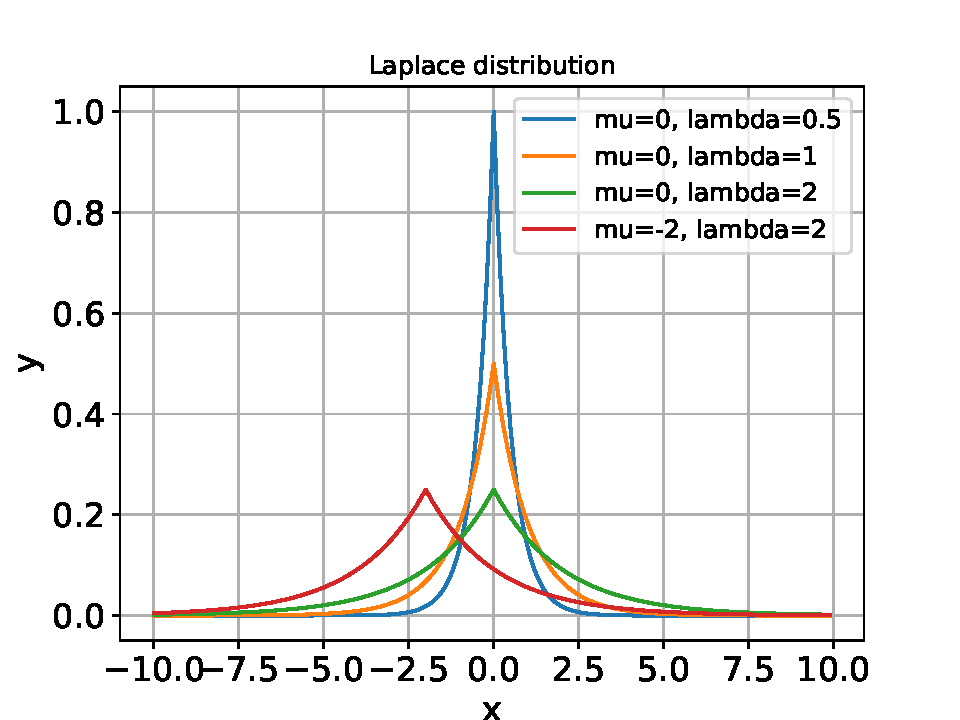
\includegraphics[scale=0.6]{\pref/LaplaceDist.pdf}
    
    \lhysays{重画}
    \caption{Laplace分布的密度函数图像}
    \label{fig:Laplace-distribution}
\end{figure}

下面我们来陈述Laplace机制。我们想利用Laplace分布来创造一些随机性. 给定一个数据集$x \in \mathcal X^n$ 和参数$\epsilon$. 对于一个算法$f:\mathcal X^n \to \R$,先计算出$f$的全局灵敏度$\mathsf{GS}_f$。输出$A_{\mathsf{Lap}}(\epsilon, x) = f(x) + Z$,其中$Z\sim \mathsf{Lap}(0, \mathsf{GS}_f/\epsilon)$. 将随机算法$A_{\mathsf{Lap}}(\epsilon, \cdot)$称为\emph{Laplace机制}\index{Laplace机制}。我们有以下定理:
\begin{theorem}\label{thm:laplace-mechanism}
    对于任意的$\epsilon > 0$,Laplace机制是$\epsilon$-DP算法.
\end{theorem}
\begin{proof}
设$x$,$x'$是两个$1$-相邻数据集,记$\mu = f(x)$,$\mu' = f(x')$. 由Laplace分布的性质可知,$A_{\mathsf{Lap}}(\epsilon, x) \sim \mathsf{Lap}(\mu, GS_f/\epsilon)$,$A_{\mathsf{Lap}}(\epsilon, x') \sim \mathsf{Lap}(\mu', GS_f/\epsilon)$.

因此,对于任意的$y \in \mathcal Y$,有
    \[
    \begin{aligned}
        \frac{h_{x}(y)}{h_{x'}(y)} &=\exp \left(-\epsilon \frac{|\mu - y| - |\mu' - y|}{GS_f} \right) \\
        &\leq \exp \left(\epsilon \frac{|\mu - \mu'|}{GS_f} \right)\leq \exp(\epsilon).
    \end{aligned}
    \]
根据\Cref{prop:continuous-dp},命题得证。
\end{proof}

\subsection{DP版本Llyod算法}
作为一个Laplace机制的具体实例,我们将$k$-均值聚类问题的经典算法Llyod算法改造成一个差分隐私算法.

\emph{$k$-均值}\index{$k$-均值}聚类问题指的是给定一个数据集$x$,找到$k$个点(中心)$\{c_i\} \subseteq \R^d$,使得$\sum_{i \in [n]} \min_{j\in[k]} \norm{x_i - c_j}^2$最小. 通俗来说,就是找到$k$个中心,使得数据集中每个点到最近的中心的距离之和最小. $k$-均值问题最常见的解决方法是使用迭代的启发式的\emph{Lloyd算法}\index{Lloyd算法},其表述为下:\lhysays{改成算法模板}
\begin{itemize}
    \item 输入:数据集$x \in \mathcal X^n$,这里$\mathcal X = \{x \in \R^d : \norm{x}_1 \leq 1 \}$,参数$k$.
    \item 随机初始化$c_1^{(0)}$, $c_2^{(0)}$, $\cdots$, $c_k^{(0)} \in \mathcal X$.
    \item for $t=1$ to $T$
    \begin{itemize}
        \item for $j=1$ to k
        \begin{itemize}
            \item 计算$S_j = \{i : c_{j}^{(t-1)} \text{ 是\ } x_i \text{ 最近的中心}\}$.
            \item 更新$c_j^{(t)} = \frac1{|S_j|}\sum_{i\in S_j} x_i$.
        \end{itemize}
    \end{itemize}
    \item 输出:$c_1^{(T)}$, $c_2^{(T)}$, $\cdots$, $c_k^{(T)}$.
\end{itemize}

这个算法可以达到很好的效果,但它并不能保证DP性质. 我们希望对这一算法进行小规模的修改,让它具有$\epsilon$-DP的性质. 我们给出如下的DP版本Llyod算法. \lhysays{改成算法模板}

\begin{itemize}
    \item 输入:数据集$x \in \mathcal X^n$,这里$\mathcal X = \{x \in \R^d : ||x||_1 \leq 1 \}$,参数$k$,\textcolor{red}{参数$\epsilon$}.
    \item \textcolor{red}{$\epsilon' = \frac{\epsilon}{2 T}$},随机初始化$c_1^{(0)}$, $c_2^{(0)}$, $\cdots$, $c_k^{(0)} \in \mathcal X$.
    \item for $t=1$ to $T$
    \begin{itemize}
        \item for $j=1$ to k
        \begin{itemize}
            \item 计算$S_j = \{i : c_{j}^{(t-1)} \text{ 是 } x_i \text{ 最近的中心}\}$.
            \item $n_j = |S_j|$.
            \item $a_j = \sum_{i\in S_j} x_i$.
            \item \textcolor{red}{计算 $\hat{n_j} = n_j + Y$,$Y \sim \mathsf{Lap}(0, 2/\epsilon')$.}
            \item \textcolor{red}{计算 $\hat{a_j} = a_j + (Z_1, \cdots, Z_d)$,$Z_i \text{ i.i.d.}\sim \mathsf{Lap}(0, 2/\epsilon')$.}
            \item 更新
            $\begin{aligned}
            c_j^{(t)} =
            \begin{cases}
                \textcolor{red}{\frac{\hat{a_j}}{\hat{n_j}}}, & \hat{n_j} \geq 1, \\
                \mathcal X\text{ 上的一个随机均匀采样}, & \hat{n_j} < 1.
            \end{cases}
            \end{aligned}$
        \end{itemize}
    \end{itemize}
    \item 输出:$c_1^{(T)}$, $c_2^{(T)}$, $\cdots$, $c_k^{(T)}$.
\end{itemize}

以下定理表明上面的算法确实是一个$\epsilon$-DP算法。
\begin{theorem}
    DP 版本的 Lloyd算法是$\epsilon$-DP算法.
\end{theorem}

\begin{proof}[证明概要]
我们只在这里陈述证明的大致想法,将细节留到习题\lhysays{习题}.

在第一步中,我们设置了$\epsilon' = \epsilon / 2 T$. 我们把整体的算法拆成$T$个阶段,其中第$t$轮迭代$A_t$以$c_1^{(t-1)},c_2^{(t-1)},\dots,c_k^{(t-1)}$作为输入,输出$c_1^{(t)},c_2^{(t)},\dots,c_k^{(t)}$. 如果可以得到$A_t$是$2 \epsilon'$-DP算法,那么由DP算法的复合性,就可以得到整个算法是$T \cdot 2\epsilon'$-DP,也就是$\epsilon$-DP.

进一步,考虑证明每一个$A_t$是$2 \epsilon'$-DP算法. 将$A_t$内循环的每一轮(以$j$为变量)视为输入为$n_j,a_j$,输出为$\hat{n}_j$,$\hat{a}_j$的算法. 分别证明这些算法符合$2\epsilon'$-DP,然后再次借助DP算法的复合性.
\end{proof}

\section{差分隐私与信息论}
\lhysays{讨论信息论约束下的差分隐私问题}

\section{习题}

\section{章末注记}

\endgroup